\documentclass[a4paper]{article}
\usepackage[utf8]{vietnam}
\usepackage{scrextend}
\changefontsizes{13pt}
\usepackage{xcolor}
\usepackage{titlesec}
\usepackage{mdframed}
\usepackage{amsmath}
\usepackage{array}
\usepackage[amsmath,standard,thmmarks]{ntheorem}
\usepackage{amssymb}
\usepackage{exscale}
\usepackage{amsfonts}
\usepackage{eucal}
\usepackage{enumerate}
\usepackage{enumitem}
\usepackage{commath}
\usepackage{graphicx}
\usepackage{tcolorbox}
\usepackage{url}
\usepackage[unicode]{hyperref}
\newmdenv[linecolor=black,skipabove=\topsep,skipbelow=\topsep,
leftmargin=-5pt,rightmargin=-5pt,
innerleftmargin=5pt,innerrightmargin=5pt]{mybox}
\setlength{\parindent}{0pt}
 \usepackage[left=2cm,right=2cm,top=2.5cm,bottom=2.5cm]{geometry}
\renewcommand{\baselinestretch}{1.5}
\newcommand{\heva}[1]{\left\{ 
\begin{aligned}#1\end{aligned}\right.}

\theoremstyle{nonumberplain} 
\theoremheaderfont{\itseries\slshape} 
\theorembodyfont{\normalfont}
\theoremsymbol{\ensuremath{_\blacksquare}} 
\renewtheorem{proof}{Chứng minh:}
\newcommand{\chm}[1]{\begin{proof}#1\end{proof}}

\usepackage{fancyhdr}
\pagestyle{fancy}
\fancyhf{}
\lhead{BTL2 - Mô hình hóa thống kê}
\cfoot{\thepage}
\rhead{Nhóm 4}
\title{BÀI TẬP LẦN 2 - MHHTK}

\author{NHÓM 4}

\date{\today}%

\begin{document}

\begin{titlepage}
\thispagestyle{empty}
\begin{center}
\textbf{\large{TRƯỜNG ĐẠI HỌC KHOA HỌC TỰ NHIÊN TP.HCM}\\
CAO HỌC KHÓA 30}\\
---------------*---------------
\end{center}
\vspace{0.3cm}
\begin{center}

\includegraphics[scale=0.8]{Logo-Math-CS.png} 
\end{center}
\vspace{0.7cm}
\begin{center}
\textbf{\Large{\textcolor[rgb]{1.0,0.0,0.0}{Bài tập lần 2}}}\\
\vspace{0.5cm}
\textbf{\Large{\textcolor[rgb]{1.0,0.0,0.0}{MÔ HÌNH HÓA THỐNG KÊ}}}\\
\vspace*{4cm}
$\begin{array}{rl}
\text{\large{Giảng viên hướng dẫn:}} &\text{\large{\bf TS. Nguyễn Thị Mộng Ngọc}}  \\
\vspace*{1cm}
\text{\large{Nhóm thực hiện:}}     & \text{\large{\textbf{Nhóm 4}}}
\end{array}$\\
\vspace{4cm}
\normalsize{TP. Hồ Chí Minh $-$ Tháng 01, 2021}
\end{center}
\end{titlepage}

\newpage
\thispagestyle{empty}
\begin{center}
\textbf{\large{BẢNG PHÂN CÔNG CÔNG VIỆC}\\}
\vspace{1cm}
\begin{tabular}{|m{4.5cm}||m{8cm}|m{3.5cm}|} 
\hline
\textbf{Thành viên} & \centering{\textbf{Công việc}} & \textbf{Mã số học viên}\\
\hline
1. Đặng Khánh Thi & $-$ & \\
& $-$  & \hspace{0.75cm}20C29038 \\
& $-$ & \\
\hline
2. Đinh Thị Nữ  & $-$ & \\
& $-$ & \hspace{0.75cm}20C29013\\
& $-$ & \\
\hline 
3. Lý Phi Long & $-$ & \\
& $-$ & \hspace{0.75cm}20C29028\\
& $-$ & \\
\hline
4. Phan Thị Thùy An & & \\
\hspace{1cm}(Nhóm trưởng) & $-$  & \hspace{0.75cm}20C29002 \\
& $-$  & \\
\hline
\end{tabular}
\end{center}

\newpage
\section*{BÀI 1}
- $X_1$: áp lực công việc\\
- $X_2$: kỹ năng quản lý\\
- $X_3$: mức độ hài lòng với chức vụ của mình\\
- $Y$: mức độ lo lắng (biến phụ thuộc)\\
Bảng ANOVA:
\begin{center}
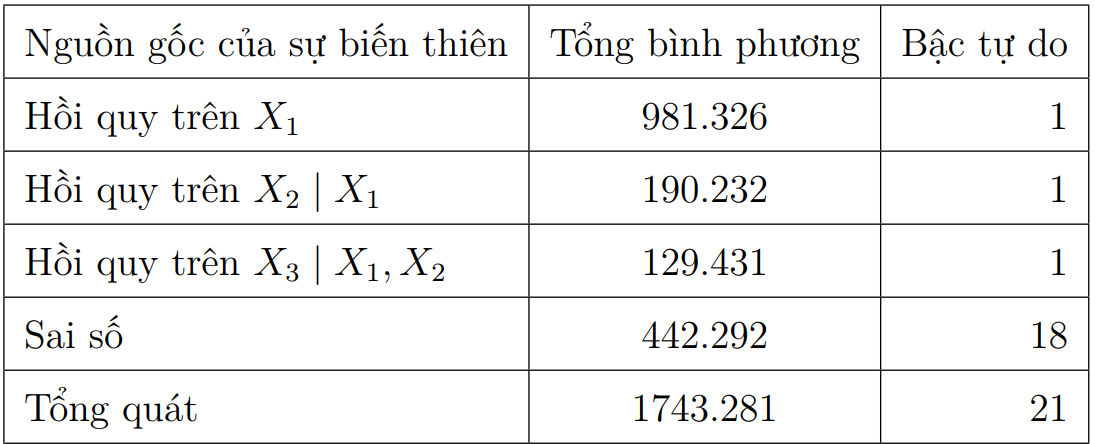
\includegraphics[scale =0.5]{anova1.PNG} 
\end{center}
\subsubsection*{1. Tính tổng bình phương hồi quy trên $X_1, X_2$ và $X_3$?}
$SSR = SSR_{X_1} + SSR_{X_2|X_1} + SSR_{X_3|X_1,X_2} = 981.326 + 190.232 + 129.431 = 1299.989$
\subsubsection*{2. Xác định tỷ lệ phần trăm sự biến thiên của mức độ lo lắng được giải thích bởi các biến
độc lập.}

\subsubsection*{3. Có thể kết luận rằng trong tất cả ba biến giải thích đều có ảnh hưởng đáng kể đến mức
độ lo lắng hay không? Chỉ rõ kiểm định nào được dùng.}

\subsubsection*{4. Nếu chúng ta chỉ xét biến giải thích $X_1$, hãy lập bảng ANOVA ?}


\subsubsection*{5. Kiểm định giả thiết sau với mức ý nghĩa 5\%}


\textbf{(a)} $H_0 : \beta_1 = 0$ \textbf{cho mô hình } $Y = \beta_0 + \beta_1 X_1 + \epsilon $


\textbf{(b)} $H_0 : \beta_2 = 0$ \textbf{cho mô hình } $Y = \beta_0 + \beta_1 X_1 + \beta_2 X_2 + \epsilon $


\textbf{(c)} $H_0 : \beta_3 = 0$ \textbf{cho mô hình } $Y = \beta_0 + \beta_1 X_1 + \beta_2 X_2 + \beta_3 X_3 + \epsilon $

\subsubsection*{6. Xác định hệ số xác định cho mỗi mô hình trong câu 5.}

\subsubsection*{7. Trong các mô hình trên, mô hình nào thích hợp nhất để giải thích sự biến động mức độ lo lắng của các giám đốc ?}



\newpage
\section*{BÀI 2}
- $Y$ : mức độ bền dẻo của nhựa\\
- $X_1$: độ dày của vật liệu\\
- $X_2$: mật độ của vật liệu
\subsubsection*{1. Tìm 2 phương trình đường thẳng hồi quy và 1 phương trình siêu phẳng (nếu có) ?}

\subsubsection*{2. Xác định tỷ lệ phần trăm sự biến thiên của biến phụ thuộc cho từng mô hình có thể có trên.}


\subsubsection*{3. Nếu chúng ta chỉ quan tâm đến cả 2 biến giải thích, hãy lập bảng ANOVA?}

\subsubsection*{4. Kiểm định giả thiết sau với mức ý nghĩa 5\%}
$$H_0 : \beta_1 = \beta_2= 0 $$

\subsubsection*{5. Xác định khoảng tin cậy với mức ý nghĩa 5\% cho $\beta_1$ trong trường hợp mô hình chỉ có biến độc lập là độ dày của vật liệu ($X_1$).}


\subsubsection*{6. Với khoảng tin cậy vừa tìm được ở câu 5, chúng ta có thể khẳng địng rằng hồi quy tuyến tính là có ý nghĩa giữa mức độ bền dẻo của nhựa và độ dày của vật liệu và mật độ của vật liệu không? Chứng minh điều khẳng định của bạn.}


\newpage
\section*{BÀI 3}


\subsubsection*{1. Viết các mô hình tuyến tính với 2 biến độc lập (có thể).}


\subsubsection*{2. Ước lượng các hệ số hồi quy trong từng mô hình tuyến tính ở câu 1.}


\subsubsection*{3. Với độ tin cậy 95\%, tìm khoảng tin cậy cho các tham số trong mô hình với 2 biến độc lập $x_1$ và $x_2$.}


\subsubsection*{4. Xác định hệ số xác định cho mỗi mô hình trong câu 1.}


\subsubsection*{5. Trong các mô hình trên, mô hình nào thích hợp nhất để giải thích sự biến thiên của $Y$ ?}


\subsubsection*{6. Viết mô hình tuyến tính dưới dạng ma trận với số biến độc lập nhiều nhất có thể, và xác định kích thước của ma trận.}


\subsubsection*{7. Ước lượng các hệ số hồi quy trong mô hình tuyến tính ở câu 6.}


\subsubsection*{8. Trong mô hình tuyến tính ở câu 6, tính ước lượng của $\mathbb{V}(\epsilon)$ và $\mathbb{V}(\hat{\beta})$.}


\subsubsection*{9. Với độ tin cậy 95\%, tìm khoảng tin cậy cho $\mathbb{V}(\epsilon)$. }


\subsubsection*{10. Khi thêm 2 biến độc lập $x_3$ và $x_2$ vào mô hình chỉ với 1 biến độc lập $x_1$ thì làm cho chất
lượng ước lượng cao hơn không?}
\end{document}
